\subsection{M4 Aggregation}
M4 is a value preserving aggregation strategy for time series data.
\begin{figure}[h]
	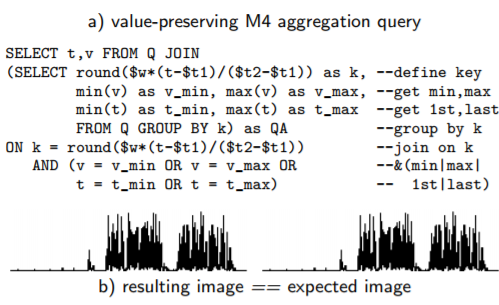
\includegraphics[width=0.5\textwidth]{m4}
	\caption{M4 query and visualization}   
	\label{fig:2}
\end{figure}
It divides the entire time series dataset into $w$ equal groups and thus each pixel column in the visualization takes only one group. For each group M4 select the aggregates $min(v)$,
$max(v)$, $min(t)$,$max(t)$ and that is why it is called M4 aggregation and then it joins the aggregated data to the time series and add missing timestamps $t_{bottom}$,$t_{top}$ and missing values $v_{first}$, $v_{last}$. In Figure \ref{fig:2} an example M4 query and 
the corresponding visualization is shown.

\textbf{Complexity of M4}: The grouping and computation of aggregated values can be done in $O(n)$ time where n is the number of tuples in the original query $Q$. Then the sub-sequent joining of the $4.w$ aggregated tuples with $Q$ requires $O(n+ 4.w)$ using hash join.